\documentclass{report}

\usepackage{fullpage}
\usepackage[skip=4pt]{caption} % ``skip'' sets the spacing between the figure and the caption.
\usepackage{pgfplots}   % Needed for plotting
\usepackage{amsmath}    % Allows for piecewise functions using the ``cases'' construct
\usepackage{graphics}   % Allows figures in the document.
\graphicspath{{img/}}
\usepackage{multicol}   % Used for two column lists

\usepackage{listings}   % Format code in the paper.
\lstset{language=Python}  

\usepackage[obeyspaces,spaces]{url} % Used for typesetting with the ``path'' command
\usepackage[hidelinks]{hyperref}   % Make the cross references clickable hyperlinks
\usepackage[bottom]{footmisc} % Prevents the table going below the footnote


% Set up page formatting
\usepackage{fancyhdr} % Used for every page footer and title.
\pagestyle{fancy}
\fancyhf{} % Clears both the header and footer
\renewcommand{\headrulewidth}{0pt} % Eliminates line at the top of the page.
\fancyfoot[LO]{CMPS242 \textendash{} Homework \#3} % Left
\fancyfoot[CO]{\thepage} % Center
\fancyfoot[RO]{Sherman \& Hammoudeh} %Right

\renewcommand\thesection{\arabic{section}} % Prevent chapter number in section number.


% Change interline spacing.
\renewcommand{\baselinestretch}{1.1}
\newcommand{\norm}[1]{\left\lVert#1\right\rVert}


\newcommand{\xvec}{\mathbf{x}}
\newcommand{\xtensor}{\mathbf{X}}
\newcommand{\y}{\mathbf{y}}
\newcommand{\w}{\mathbf{w}}
\newcommand{\wstar}{\mathbf{w}^{\star}}
\newcommand{\T}{^\textrm{T}}
\newcommand{\wTx}{\w^{\T}\xvec}
\newcommand{\wTxi}{\w^{\T}\xvec_{i}}
\newcommand{\yhat}{\hat{\mathbf{y}}}


\title{\textbf{CMPS242 Homework \#3 \textendash{} Logistic Regression}}
\author{Benjamin Sherman \\~\\ \& \\~\\ Zayd Hammoudeh}


\begin{document}
  \maketitle
  
  \suppressfloats
  \section{Homework Objective}
  
  Develop a logistic regression-based learner that can identify SMS text messages as either SPAM or ham (i.e.,~not SPAM).  Additional requirements include:
  
  \begin{itemize}
    \setlength\itemsep{0pt}
    \item Learner should implement a batch gradient descent
    \item Create a Jupyter (i.e., IPython) notebook to document all work
  \end{itemize}

  \noindent
  Four extra credit tasks were also possible for this homework.  They are:
  
  \begin{enumerate}
    \setlength\itemsep{0pt}
    \item Support a bias term in the weight vector~($\mathbf{w}$) that is not regularized
    \item Experiment with different regularizers, such as~$\lambda\norm{\w}_1$.
    \item Implement the stochastic gradient descent algorithm
    \item Implement the exponentiated gradient algorithm (EG\textsuperscript{$\pm$})
  \end{enumerate}
 
  \section{Gradient Descent Update Rule}
  
  Logistic regression is a subcategory of binary classification.  Define the logistic (sigmoid) function as shown in Eq.~\eqref{eq:logisticFunction}.
  
  \begin{equation}
    \sigma(a) = \frac{e^{a}}{1+e^{a}}\label{eq:logisticFunction}
  \end{equation}
  
  \noindent
  As shown in Figure~\ref{fig:sigmoidGraph}, this function is bounded between~$0$ and~$1$ making it ideal for binary classification since it can be used to represent probabilities without additional normalization. The following notes show the derivation of the logistic update rule.\footnote{This proof is based on the \href{http://cs229.stanford.edu/notes/cs229-notes1.pdf}{lecture notes of Andrew Ng}.}
  
  \begin{figure}[tb]
    \centering
    \begin{tikzpicture}[scale=0.5]
      \hspace{-0.3in}
      \begin{axis}[ 
        xmin=-10,
        xmax=10,
        xlabel=$a$,
        ylabel={$\sigma(a)$}
        ] 
        \addplot[smooth, color=blue, domain=-10:10] {(exp(x)/(1+exp(x))}; 
      \end{axis}
    \end{tikzpicture}
    \caption{Plot of the Logistic Function}\label{fig:sigmoidGraph}
  \end{figure}

  Define Z as a random variable that maps one classification value (e.g.,~ham) to~$0$ and the other classification result (e.g.,~SPAM) to~$1$.  We could then define the probability of a~$0$ or a~$1$ as shown in Eq.~\eqref{eq:prZeroSigma} and~\eqref{eq:prOneSigma} respectively.  This can be written compactly as shown in Eq.~\eqref{eq:prGenericSigma}.
  
  \begin{align}
    \Pr\{Z=0|a\}&=1-\sigma(a)\label{eq:prZeroSigma}\\
    \Pr\{Z=1|a\}&=\sigma(a)\label{eq:prOneSigma}\\
    \Pr\{Z=z|a\}&=\sigma(a)^{z}(1-\sigma(a))^{1-z}\label{eq:prGenericSigma}
  \end{align}
 
  \noindent
  Given a target classification vector~$\y$ and the relation~$a=$, the likelihood~($L$) is in turn defined as shown in Eq.~\eqref{eq:likelihoodJoint}.  Since each element is independent, this probability can be transformed into a product as shown in Eq.~\eqref{eq:likelihoodIndependent}, where~$n=|\y|$.
  
  \begin{align}
    L(\w)&=\Pr\{\y | \wTx \}\label{likelihoodJoint}\\
        &=\prod_{i=1}^{n}\Pr\{y_i | \wTxi \}\label{eq:likelihoodIndependent}
  \end{align}
 
  As with homework~\#1, the value that maximizes the likelihood of a non-negative function also maximizes the log likelihood.  Hence, Eq.~\eqref{eq:likelihoodIndependent} can be transformed to Eq.~\eqref{eq:logLikelihood}.
  
  \begin{align}
    \ln L(\w) &= \ln \left(\prod_{i=1}^{n}\Pr\{y_i | \wTxi\}\right)\\
             &= \sum_{i=1}^{n}\ln \Pr\{y_i | \wTxi\}\\
             &= \sum_{i=1}^{n}\ln \left( \sigma(\wTxi)^{y_i} (1-\sigma(\wTxi))^{1-y_i} \right)\\
             &= \sum_{i=1}^{n} \ln \left(\sigma(\wTxi)^{y_i}  + \ln \left( (1-\sigma(\wTxi))^{1-y_i} \right) \right)\\
             &= \sum_{i=1}^{n} y_i \ln \sigma(\wTxi) + (1-y_i) \ln (1-\sigma(\wTxi)) \label{eq:logLikelihood}
  \end{align}
 
  To find the maximizing likelihood, the derivative is taken and set equal to~$0$.  We use the identity ${\frac{\partial \sigma(a)}{\partial a} = \sigma(a)(1-\sigma(a))}$ without proof, but the proof is trivial. Hence the maximizing value is is shown in Eq.~\eqref{eq:derivLossFunction}; note that the \textit{chain rule} was used for this derivative.
  
  \begin{align}
    0 &= \sum_{i=1}^{n} \left( y_i \frac{1}{\sigma(\wTxi)} \frac{\partial \sigma(\wTxi)}{\partial \w} - (1-y_i) \frac{1}{1-\sigma(\wTxi)} \frac{\partial \sigma(\wTxi)}{\partial \w} \right)\\
    &= \sum_{i=1}^{n} \left( y_i \frac{1}{\sigma(\wTxi)} \sigma(\wTxi)(1-\sigma(\wTxi))\xvec_i - (1-y_i) \frac{1}{1-\sigma(\wTxi)} \sigma(\wTxi)(1-\sigma(\wTxi))\xvec_i \right)\\
    &= \sum_{i=1}^{n} \left(y_i (1-\sigma(\wTxi)) - (1-y_i) \sigma(\wTxi) \right)\xvec_i\\
    &= \sum_{i=1}^{n} (y_i -\sigma(\wTxi))\xvec_i \label{eq:derivLossFunction}
  \end{align}
  
  Eq.~\eqref{eq:derivLossFunction} represents the maximizing gradient for the log likelihood.  This can then be substituted into the update rule for stochastic gradient descent, where $\eta$~is the hyperparameter, learning rate.
  
  \begin{equation}
    \w_{t+1}:=\w_{t}+\eta \nabla \ln L(\w)\label{eq:updateRuleGradient}
  \end{equation}
  
  \noindent
  We can then substitute into Eq.~\eqref{eq:updateRuleGradient}, using tensor notation since this is batch update.  
  
 \begin{equation}
  \w_{t+1}:=\w_{t}+\eta \xtensor^{\T}(\y -\yhat)^{\T}\label{eq:finalUpdateRule}
 \end{equation}
  
  \noindent
  Note that that~$\w_{t}$ was used in the gradient since it is not known how to maximize on $w_{t+1}$.  In addition, the learning rate,~$\eta$ uses a constant configured by the user an aging term as shown in Eq.~\eqref{eq:learningRate}.
   
  \begin{equation}
    \eta = \frac{\eta_0}{t^{0.9}}
    \label{eq:learningRate}
  \end{equation}
  
  \noindent
  Our implementation uses the update rule and learning rate in Eq.~\eqref{eq:finalUpdateRule} and~\eqref{eq:learningRate} respectively for all batch gradient descent experiments in this paper.
    
  \section{Text Preprocessor}
  
  Before learning can be attempted the natural language text in the form of SMS messages much be turned into a feature vectors.  We accomplish this through a multistep process described below (in order).

  \begin{itemize}
    \item \textit{Import CSV File} -- Pandas' native CSV~support as part of the \texttt{DataFrame} object was used.
    \item \textit{Invalid Character Removal} -- The original text files (before my team cleaned them for the class) had invalid, unsupported characters.  We cleaned the 
    \item \textit{Punctuation Removal} -- The punctuation set is defined by Python's \texttt{string} package (i.e.,~``string.punctuation'').  Punctuation removal entailed replacing all punctation symbols with the empty string (e.g.,~``couldn't'' became~``couldnt'').
    \item \textit{Capitalization Correction} -- Standardizes case so that words with different capitalization are not treated differently.
    \item \textit{Stop Words Removal} -- The set of ``stop words'' is non-standard.  For our experiments, we used the English ``\texttt{corpus}'' dictionary bundled with the Natural Language Toolkit (NLTK).
  \end{itemize}

  \section{Jupyter Notebook Implementation}
  
  Jupyter notebooks serve as a intermediary layer that insulates users from the underlying code implementation.  We included multiple features into our Jupyter notebook to improve the user experience and provide external learner configuration and data visualization.
  
  \subsection{Specifying Hyperparameters}
  
  Since Jupyter notebook masks the code from the user, some may find it difficult to experiment with different configurations.  To address this limitation, we added a series of widgets to our notebook.  They leverage the \texttt{ipywidgets} library.  The specific hyperparameters that are controllable by widgets are:
  
  \begin{itemize}
    \setlength\itemsep{0pt}
    \item Cross-validation fold count ($k$)
    \item Learning algorithm (e.g.,~standard gradient descent, exponentiated gradient descent, and stochastic gradient descent)
    \item Regularizer selection (e.g.,~$L_2$ or~$L_1$~norm)
    \item Error calculation formula (e.g.,~$1 - Accuracy$ or root-mean square)
    \item Maximum number of training epochs
    \item Learning rate~($\alpha$)
    \item $\lambda$~range -- These are the powers of~$2$ to test.
  \end{itemize}
  
  Figure~\ref{fig:jupyterWidgets} shows a screenshot from our Jupyter notebook with the widgets included.
    
  \begin{figure}[tb]
    \centering
    \fbox{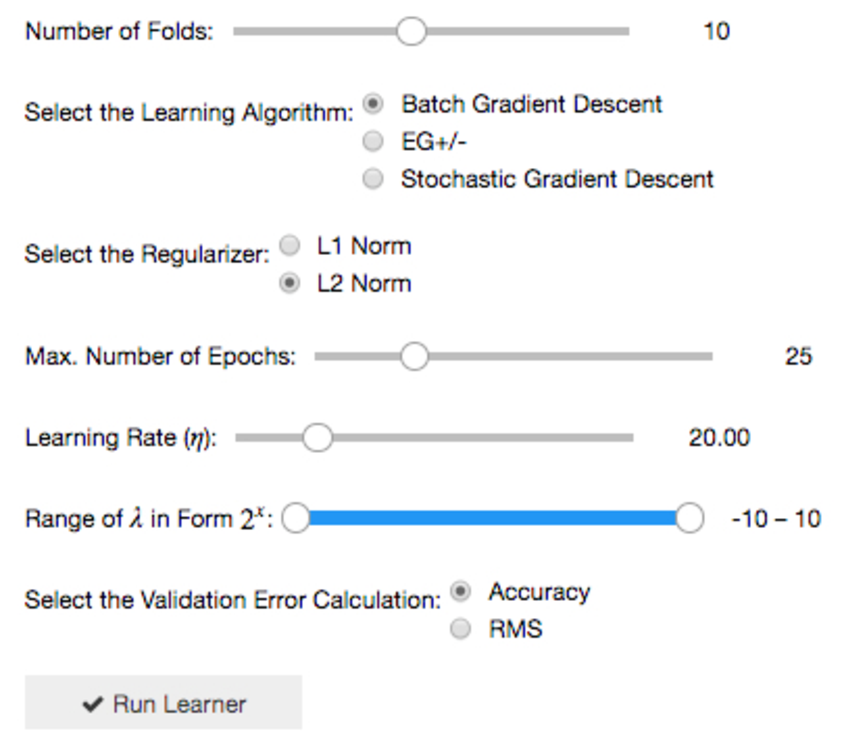
\includegraphics[scale=.3]{jupyter_widgets}}
    \caption{Jupyter notebook experiment configuration widgets}\label{fig:jupyterWidgets}
  \end{figure}

  \subsection{Learner Progress Indicator}
  
  As with most iterative learning algorithms, our learner does provide instantaneous results.  Depending on the user specified configuration described in the previous section, it may take several minutes before a run of the algorithm completes.  Our implementation provides visual feedback on the learners progress via a text-based progress bar, which is shown in Figure~\ref{fig:jupyterProgressBar}.\footnote{The underlying implementation used for this feature was from an online resource and not developed natively by our team.}
  
  \begin{figure}[tb]
    \centering
    \fbox{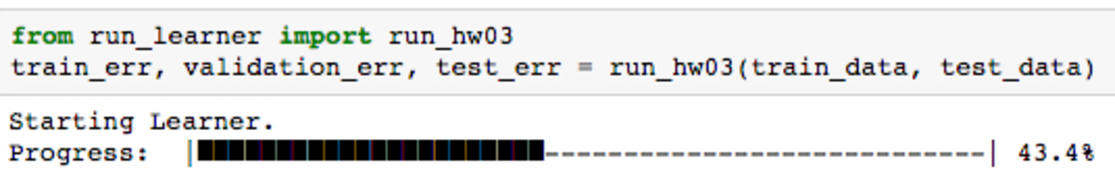
\includegraphics[scale=.3]{jupyter_progress_bar}}
    \caption{Jupyter notebook learner progress indicator}\label{fig:jupyterProgressBar}
  \end{figure}

  \subsection{Embedded Results Table}
  
  To improve the Jupyter notebook experience, we built in support for a table that will display the latest execution's results.  The minimum training, validation and test errors are bolded and highlighted in yellow as shown in Figure~\ref{fig:jupyterTable}.
    
  \begin{figure}[tb]
    \centering
    \fbox{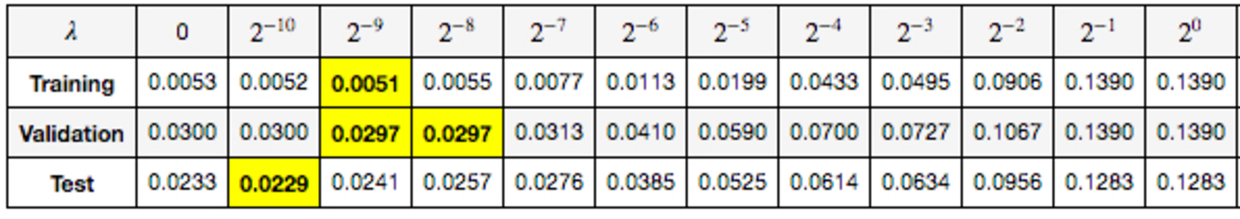
\includegraphics[scale=.5]{jupyter_table}}
    \caption{Example Jupyter notebook table of experimental results}\label{fig:jupyterTable}
  \end{figure}
  
  \subsection{Embedded Result Graphing}
  
  We also implemented graphing into our Jupter notebook.  This uses Python's \texttt{matplotlib} package.  An example graph is shown in Figure~\ref{fig:jupyterGraph}.
  
  \begin{figure}[tb]
    \centering
    \fbox{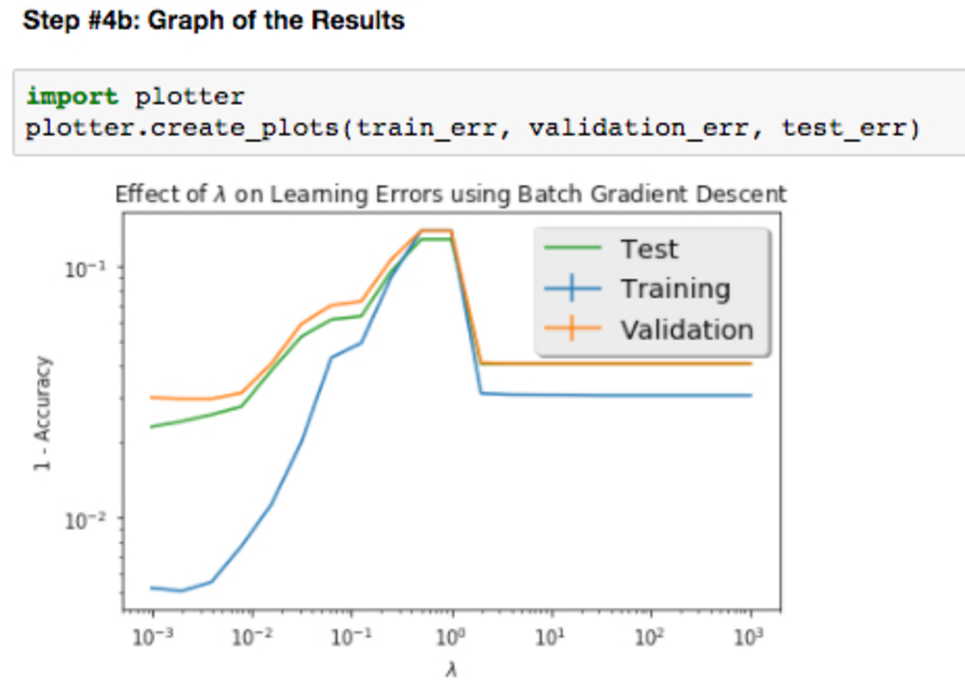
\includegraphics[scale=.5]{jupyter_graph}}
    \caption{Example Jupyter notebook graph of experimental results}\label{fig:jupyterGraph}
  \end{figure}

  
  \section{Experiment Setup}\label{sec:experimentSetup}
  
  Our solver is implemented in Python 2.7.13.  It requires a set of external packages, including: 
  
  \begin{multicols}{2}
    \begin{itemize}
      \setlength\itemsep{0pt}
      \item Pandas
      \item Scikit-Learn
      \item NumPy
      \item IPython
      \item Matplotlib
      \item ipywidgets\textrm{.}
    \end{itemize}
  \end{multicols}

  The default experiment setup was:
  
  \begin{itemize}
    \item \textit{Performance Metric}: Accuracy which rounds~$\yhat$ to the closest integer.
    \item \textit{Learning Algorithm}: Batch gradient descent
    \item \textit{Regularizer}: $L_2$ norm
    \item \textit{Cross-validation Fold Count ($k$)}: 10
    \item \textit{Number of Training Epochs/Rounds}: 15
    \item \textit{$\lambda$ Range}: $0,2^{-10},2^{-9},...,2^{9},2^{10}$
    \item \textit{Learning Rate ($\eta_0$)}: 20
    \item \textit{Graph Error Bars}: These are included in all graphs.  However, the variance between folds is low meaning they are often not visible.
  \end{itemize}

  \section{Extra Credit \#1: Bias Term Support}
  
  A bias term in the learning algorithm can only improve the learner's performance by accounting for shifts in the data.  As such, our implementation only supports training with a bias; we deliberately chose that this feature could not be disabled.  
  
  The bias term is added to the input tensor,~$X$, as a column of value $1$.  This is done using NumPy.  When calculating the regularization error, we ignore the error caused by the bias term by setting its error to~$0$ as shown in Figure~\ref{fig:codeBiasRegularizerRemoval}.
  
  \begin{figure}[tb]
    \begin{lstlisting}[frame=single] 
      def l2_norm_regularizer(lambda_val, w):
        reg_err = np.multiply(lambda_val, w)
        reg_err[0, 0] = 0  # Exclude the bias
        return reg_err
    \end{lstlisting}
    \caption{Implementation of Bias Regularizer Error Removal}\label{fig:codeBiasRegularizerRemoval}
  \end{figure}

  \section{Batch Gradient Descent Learning Performance}
  
  Our batch gradient descent implementation followed the experiment setup described in Section~\ref{sec:experimentSetup}.  The best error was observed when there was no regularizer as shown in Table~\ref{tab:batchGradientDescentL2} and Figure~\ref{fig:batchGdL2}.  It is also important to note that as the regularizer increased, the error drops precipitously and remains largely unchanged.  This occurs because the regularizer begins to saturate the sigmoid function causing it to return a $yhat$ of~$0$ for all but the most obvious cases of spam.
    
  \begin{table}[]
    \centering
    \caption{Effect of the $L_2$ Regularizer on Batch Gradient Descent Performance}
    \label{tab:batchGradientDescentL2}
    \begin{tabular}{c|c|c|c|c|c|c|c|c|c|c}
      \hline
      $\lambda$  & 0              & $2^{-10}$ & $2^{-9}$ & $2^{-8}$       & $2^{-7}$ & $2^{-6}$ & $2^{-5}$ & $2^{-4}$ & $2^{-3}$ & $2^{-2}$ \\ \hline
      Training   & 0.008          & 0.007     & 0.007    & \textbf{0.006} & 0.008    & 0.013    & 0.023    & 0.043    & 0.058    & 0.099    \\ \hline
      Validation & \textbf{0.027} & 0.028    & 0.029    & 0.029          & 0.032    & 0.039    & 0.057    & 0.072    & 0.081    & 0.113    \\ \hline
      Test       & \textbf{0.024} & 0.024     & 0.024    & 0.026          & 0.028    & 0.034    & 0.051    & 0.060    & 0.061    & 0.098    \\ \hline
    \end{tabular}
  \end{table}


  \begin{figure}
    \centering
    \includegraphics[scale=.3]{batch_GD_L2Norm}
    \caption{Effect of regularizer~$\lambda$ on batch gradient descent performance using $L_2$ norm}\label{fig:batchGdL2}
  \end{figure}
    
  \section{Extra Credit \#2: Multiple Regularizer Experimentation}

  An extra credit portion of the assignment was to investigate the performance of the learner with another regularizer.  As the homework proposed, we use the $L_1$.  Unlike the $L_2$ from Section~\ref{}, the derivative of the $L_1$ norm is a vector of ones multiplied by~$lambda$.  As such, the value of~$\w$ does not affect the regularization.  As expected, the affect of this norm on the learner's performance is far more muted as shown in Table~\ref{tab:batchGradientDescentL1} and Figure~\ref{fig:batchGdL1}.  The clamping of the logistic function was not observed and there was not significant change in the learner's performance for small values of~$\lambda$ (i.e.,~less than~$1$).  This behavior is fully expected.

  \begin{table}[]
    \centering
    \caption{Effect of the $L_1$ Regularizer on Batch Gradient Descent Performance}
    \label{tab:batchGradientDescentL1}
    \begin{tabular}{c|c|c|c|c|c|c|c|c|c|c}
      \hline
      $\lambda$  & 0              & $2^{-10}$ & $2^{-9}$ & $2^{-8}$       & $2^{-7}$ & $2^{-6}$ & $2^{-5}$ & $2^{-4}$ & $2^{-3}$ & $2^{-2}$ \\ \hline
      Training   & \textbf{0.007} & \textbf{0.007}     & \textbf{0.007}    & 0.008 & 0.008    & 0.008    & 0.008    & 0.008    & 0.008    & 0.008    \\ \hline
      Validation & \textbf{0.030} & \textbf{0.030}    & \textbf{0.030}    & \textbf{0.030} & \textbf{0.030}    & \textbf{0.030}    & \textbf{0.030}    & 0.031    & 0.031    & 0.031    \\ \hline
      Test       & \textbf{0.024} & \textbf{0.024}     & \textbf{0.024}    & \textbf{0.024} & \textbf{0.024}    & \textbf{0.024}    & \textbf{0.024}    & \textbf{0.024}    & \textbf{0.024}    & 0.026    \\ \hline
    \end{tabular}
  \end{table}


  \begin{figure}
    \centering
    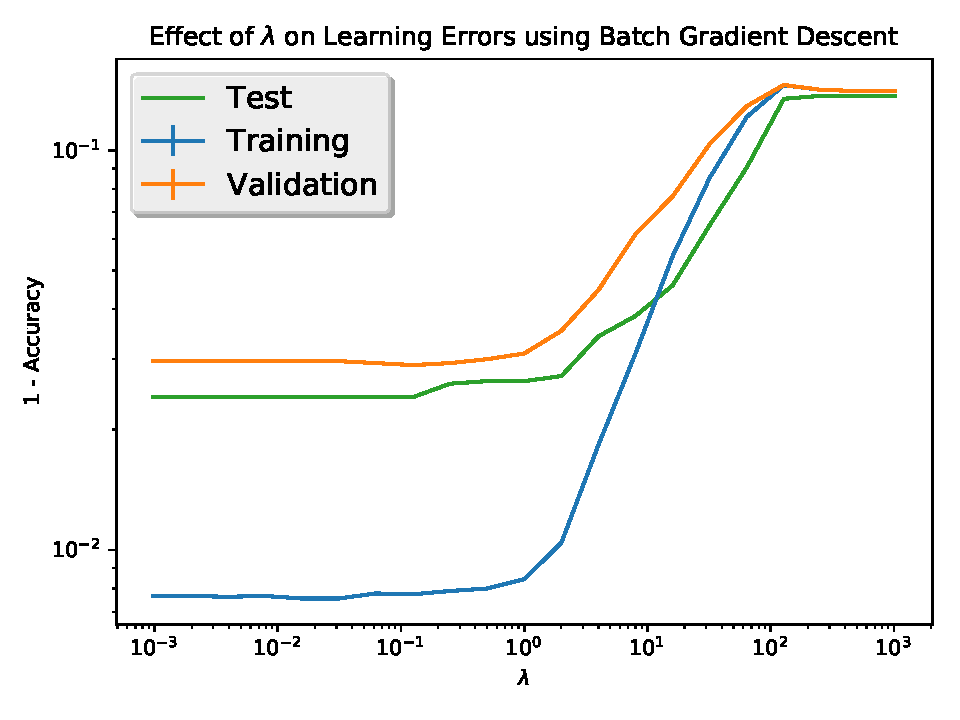
\includegraphics[scale=.5]{batch_GD_L1Norm}
    \caption{Effect of regularizer~$\lambda$ on batch gradient descent performance using $L_1$ norm}\label{fig:batchGdL1}
  \end{figure}

  \section{Extra Credit \#3: Stochastic Gradient Descent}
  
  In each training round/epoch, batch gradient descent performs a single update of the weight vector based off \textit{all} the training samples.  In contrast, given a dataset of size~$m$, stochastic gradient descent (SGD) performs $m$ updates of the weight vector in each epoch.  This generally should cause the trainer to require less epochs and train faster on average.
  
  Since a single element at a time is used to update the weight vector, the learning rate,~$\eta_{0}$ should be smaller to prevent over-correction based on a single outlier.  As such, we reduced the learning rate to~$0.1$ for this experiment.  Figure~\ref{tab:stochasticGradientDescentL2} and Table~\ref{tab:stochasticGradientDescentL2} show that SGD had better performance than batch gradient descent.  Although the selected regularizer~($2^{-10}$) did not have the minimum test error, the difference is quite small.  Like despite also using the L2 norm, SGD did not have the same clamped error for larger values of~$\lambda$.
  
  While stochastic gradient descent takes far few epochs to converge (5 versus more than~15 for batch gradient descent), the running time is actually longer for SGD by about a factor of 3~times.  This is due primarily to the inefficiencies of Python and how it interacts with NumPy.  When all the matrix multiplications are performed at once, the just-in-time (JIT) compiler is able to optimize them.  It is not able to do the same level of optimization when multiplications are made one at a time in SGD.
  
    \begin{table}[]
    \centering
    \caption{Effect of the $L_1$ Regularizer on Batch Gradient Descent Performance}
    \label{tab:stochasticGradientDescentL2}
    \begin{tabular}{c|c|c|c|c|c|c|c|c|c|c}
      \hline
      $\lambda$  & 0              & $2^{-10}$ & $2^{-9}$ & $2^{-8}$       & $2^{-7}$ & $2^{-6}$ & $2^{-5}$ & $2^{-4}$ & $2^{-3}$ & $2^{-2}$ \\ \hline
      Training   & \textbf{0}  & \textbf{0}    & \textbf{0}    & \textbf{0} & 0.001   & 0.002    & 0.005    & 0.013    & 0.024    & 0.046    \\ \hline
      Validation & 0.026 & \textbf{0.025}    & 0.029  & 0.030 & 0.030    & 0.032    & 0.032    & 0.034    & 0.040    & 0.061    \\ \hline
      Test       & \textbf{0.018} & 0.019     & 0.019    & 0.021          & 0.021    & 0.022    & 0.020    & 0.026    & 0.037    & 0.056    \\ \hline
    \end{tabular}
  \end{table}
  
  \begin{figure}
    \centering
    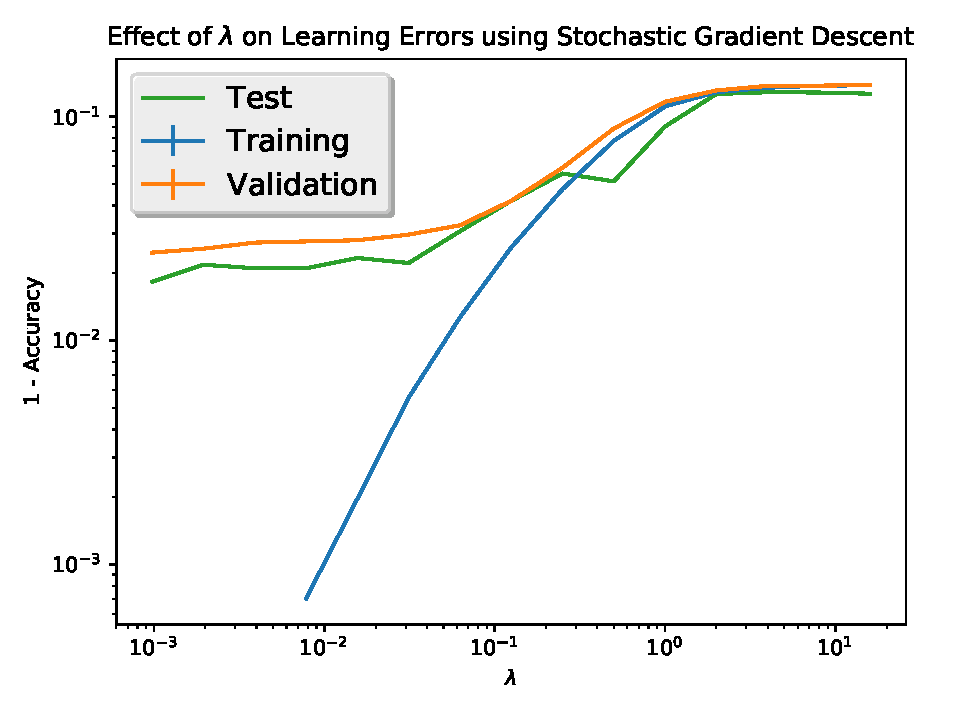
\includegraphics[scale=.5]{stochastic_GD_L2Norm}
    \caption{Stochastic Gradient Descent Performance using the $L_{2}$ norm and a learning rate of~$0.1$}\label{fig:stochasticGDL2}
  \end{figure}
    
  \section{Extra Credit \#4: Exponentiated Gradient Descent}
 
\end{document}